\chapter{Trennen}

\section{Stoffgemische}

%Tabelle START

\vspace*{-2.5mm}
\renewcommand{\arraystretch}{1.2}
\begin{table}[h!]
	\centering
	\caption{Stoffgemische}
	\label{tab:tabelle1}
	%\resizebox{10cm}{!}{
	\begin{tabulary}{\textwidth}{C|L}
		\hline
		\textbf{Kombination der Phasen} & \textbf{Bezeichnung}\\
		\hline
		S in G & Rauch, Staub,...\\
		S in L (Aerosol)& Suspension, Schlamm, Trübe,...\\
		L in G (Aerosol)& Dampfwolken, Nebel, Regen, Sprühwolke,...\\
		G in L & Sprudelschicht, Blasenschwarm, Schaum,...\\
		L in L & Emulsion, Tropfenschwarm\\
	\end{tabulary}
	%}
\end{table}
\FloatBarrier
\vspace*{-2.5mm}

%Tabelle Ende

\section{Trennverfahren}

Alle Stoffsysteme sind dispers und bestehen aus mindestens 2 Phasen.\\
Nur dann kann man \underline{mechanische Trennverfahren} anwenden. \\
(Grenze nach unten ist dabei die Partikelgröße)\\ \\
Für einphasige Stoffsysteme müssen thermische Trennverfahren angewendet werden.\\
Mechanische Verfahren sind meist effizienter als thermische Verfahren.

\begin{itemize}
	\item \textbf{Sedimentation} $\approx \SI{10}{\micro \meter}$ \begin{small}(S/G, S/L, L/L, G/L, L/G)\end{small}\\
	= Absetzen/Aufsteigen von Teilchen im Schwerkraftfeld \\ \\
	$\rightarrow$ \textit{Voraussetzung:} \\
	unterschiedliche Dichte der Teilchen gegenüber Fluid
		
	\item \textbf{Zentrifugation} $< \SI{10}{\micro \meter}$ \begin{small}(S/L)\end{small}\\
	= Trennen im Zentrifugalfeld \\ \\
	$\rightarrow$ geeignet für sehr geringe Dichteunterschiede und sehr kleine Teilchen
	
	\item \textbf{Filtration} \begin{small}(S/G, S/L)\end{small}\\
	= Teilchendurchmesser > Porendurchmesser des Filtermediums \\
	"`Sterische (räumliche) Hinderung"' 
	
	\item \textbf{Sieben} \begin{small}(S/G)\end{small}\\
	= Trennen nach Größenunterschied \\
	$\rightarrow$ Klassierung
	
	\item \textbf{Sichten} \begin{small}(S/G)\end{small}\\
	= Trennen nach Luftwiderstand und Dichte
	
	\item \textbf{Flotation} \begin{small}(S/S/G)\end{small}\\
	= spezielle Sedimentation
	
	\item \textbf{Zyklon} \begin{small}(S/G, S/L)\end{small}\\
	= ähnlich wie Zentrifugation
\end{itemize}

\subsection{Sedimentation}
= Absetzen einer dispersen Phase unter Einwirkung der Schwerkraft\\

Disperse Phase kann eine höhere oder niedrigere Dichte haben, als die Kontinuierliche.\\
$\rightarrow$ wichtige Trennoperation, weil Apparate \underline{einfach} und somit \underline{günstig} sind\\

\textbf{Bezeichnung des Sediments nach Zweck}
\begin{itemize}
	\item \textit{Klären:} \\
	Trennziel = klare Flüssigkeit mit möglichst wenig Teilchen
	\item \textit{Eindicken:} \\
	Trennziel = möglichst konzentrierter Schlamm mit möglichst wenig Flüssigkeit
\end{itemize}



\newpage

\section{Grundlagen der Modellierung}
Bewegung eines Einzelteilchens im Schwerkraftfeld\\
$\rightarrow$ Annahme: Teilchen ist starr, kugelförmig und glatt\\ \\
$d_P>\SI{10}{\micro \meter}$\\
$\rho_P>\rho_F$
\vspace*{-20mm}
%Start
\begin{figure}[h!]
	\centering
	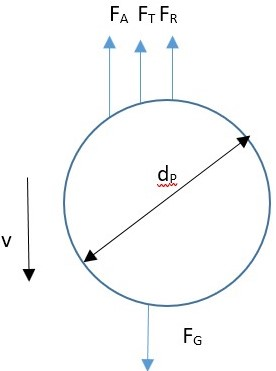
\includegraphics[width=0.22\textwidth]{img/partikelmodell}
	\caption{Skizze eines Partikels}
	\label{skizzepruef}
\end{figure}
\FloatBarrier
%Ende
\vspace*{-5mm}
\begin{flalign}
F_G &= m_P*g=V_P*\rho_P*g=\frac{\pi}{6}*d_P^3*\rho_P*g\\
F_T &= m_F*g=V_P*\rho_F*g=\frac{\pi}{6}*d_P^3*\rho_F*g
\end{flalign}
\begin{small}\begin{center}"'Auftrieb ist Masse der verdrängten Flüssigkeit"'\end{center}\end{small}
\vspace*{-5mm}
\begin{flalign}
F_R &= c_W*\rho_F*\frac{1}{2}*v_P^2*A_\perp
\end{flalign}


$c_W$... Widerstandsbeiwert $c_W=f(v,\text{Geometrie}, \text{Rauigkeit},...)$\\
$v_P$... Relativgeschwindigkeit zwischen Teilchen und Partikel\\
$A_\perp$... Projezierte Fläche des Partikels in Bewegungsrichtung\\
hier: Kugel $\rightarrow$ Kreis mit $A_\perp=\frac{\pi}{4}*d_P^2$













